\documentclass[twocolumn,epjc3]{svjour3}

\usepackage[T1]{fontenc}
%\usepackage{mathptmx}   % no bold math fonts (in title), known bug
\usepackage{newtxtext}   % text Times fonts
\usepackage{newtxmath}   % math Times fonts

\usepackage{graphicx}
\usepackage{flushend}
\usepackage{xspace}
\usepackage{cite}
\usepackage[colorlinks,citecolor=blue,urlcolor=blue,linkcolor=blue]{hyperref}

\journalname{Eur. Phys. J. A}
\graphicspath{{figures/}}

\newcommand{\np}     {\ensuremath{np \rightarrow pn}\xspace}
\newcommand{\dpfrag} {\ensuremath{dp \rightarrow ppn}\xspace}
\newcommand{\dpchex} {\ensuremath{dp \rightarrow (pp)n}\xspace}
\newcommand{\dpret}  {\ensuremath{dp \rightarrow (pn)p}\xspace}
\newcommand{\GeVc}   {Ge\kern-.1emV/c\xspace}
\newcommand{\GeV}    {Ge\kern-.1emV\xspace}

\begin{document}

\title{Charge exchange
  $\boldsymbol{{\dpchex}}$ % correct bold math fonts (not for mathptmx)
  reaction study at 1.75 A \GeVc by the STRELA spectrometer}

\author{\raggedright
  S.~N.~Basilev\thanksref{jinr}    \and Yu.~P.~Bushuev\thanksref{jinr}   \and
  S.~A.~Dolgiy\thanksref{jinr}     \and V.~V.~Glagolev\thanksref{jinr}   \and
  D.~A.~Kirillov\thanksref{jinr}   \and N.~V.~Kostyaeva\thanksref{jinr}  \and
  A.~D.~Kovalenko\thanksref{jinr}  \and A.~N.~Livanov\thanksref{jinr}    \and
  P.~K.~Manyakov\thanksref{jinr}   \and G.~Martinsk\'{a}\thanksref{upjs} \and
  J.~Musinsky\thanksref{saske}     \and N.~M.~Piskunov\thanksref{jinr}   \and
  A.~A.~Povtoreiko\thanksref{jinr} \and P.~A.~Rukoyatkin\thanksref{jinr} \and
  R.~A.~Shindin\thanksref{jinr}    \and I.~M.~Sitnik\thanksref{jinr}     \and
  V.~M.~Slepnev\thanksref{jinr}    \and I.~V.~Slepnev\thanksref{jinr}    \and
  J.~Urb\'{a}n\thanksref{upjs}
}

\institute{\noindent
  \,Joint Institute for Nuclear Research, Joliot Curie 6, 141980 Dubna,
  Moscow region, Russia\label{jinr} \and
  \,University of P.\,J. \v{S}af\'{a}rik, Jesenn\'{a} 5, 04001 Ko\v{s}ice,
  Slovak Republic\label{upjs} \and
  \,Institute of Experimental Physics, Watsonova 47, 04001 Ko\v{s}ice,
  Slovak Republic\label{saske}
}
\thankstext{e1}{\,e-mail: contact@example.com (corresponding author)}

\date{Received: date / Accepted: date}
% The correct dates will be entered by the editor
\maketitle

\begin{abstract}
  The differential cross sections of the charge exchange reaction \dpchex has
  been measured at 1.75 \GeVc per nucleon for small transferred momenta using
  the one arm magnetic spectrometer STRELA at the Nuclotron accelerator in JINR
  Dubna. The ratio of the differential cross section of the charge exchange
  reaction \dpchex to that of the \np elementary process is discussed in order
  to estimate the spin-dependent part of the \np charge exchange amplitude. The
  \np amplitude turned out to be predominantly spin-dependent.
\end{abstract}

\section{Introduction}
In the theory of nucleon-nucleon scattering extracting complex amplitudes of the
scattering matrix is a matter of fundamental importance. For all amplitudes to
be obtained, a complete experiment must be performed, \textit{i.e.}, an
experiment with a set of observed quantities providing a full and exhaustive
description of this process. Such an experiment comprises measurements with
polarized both projectile and target what is large and laborious task.

However, under certain experimental conditions, there is a possibility to
determine some amplitudes of the scattering matrix or a set of them. One of the
chances is the charge exchange reaction on the deuteron \dpchex with the use of
unpolarized protons and unpolarized deuterons, which under certain conditions is
determined only by the spin-dependent amplitude of the elementary \np
scattering. When studying the differential cross section of this reaction at
small four-momentum transfer squared, it is possible to estimate the
spin-dependent term of the \np scattering amplitude in the context of the
impulse approximation. The effect can be understood qualitatively in the
following way. Two nucleons, bound in the deuteron may be in $^3S_1$ and $^3D_1$
$(T = 0)$ spatial and spin symmetric states; their isospin is antisymmetric. In
the charge exchange at $0^\circ$ w.r.t. laboratory frame (proton rest frame),
the transition from $^3S_1$ or $^3D_1$ to a charge symmetric $^1S_0$ or $^1D_2$
state of the two protons requires spin flip, in order to satisfy the Pauli
principle and ensure an antisymmetric total wave function. In this way, the
spin-dependent part of the elementary charge exchange amplitude will be
reflected through the probability of the charge exchange process on the
deuteron.

The original idea to take use of the charge exchange reaction on the unpolarized
deuteron to determine the spin-dependent part of the \np charge exchange was
proposed by Pomeranchuk \cite{pom51} and Chew \cite{chew51}. Later this
possibility was emphasized in a series of works partly
\cite{mig55,pom51_2,lap57,dea72,dea72_2,ala75,ala75_2,bug87}. The mathematical
description was developed later by Dean \cite{dea72,dea72_2}. These formulas
were obtained under certain assumptions, namely relying on the validity of the
impulse and closure approximations. In the work by Lednicky and Lyuboshitz
\cite{led04} it was shown that at relativistic energies these two assumptions
are also justified.

In the general case the nucleon-nucleon ($NN$) amplitude in the centre of mass
system can be presented as \cite{gla02}
\begin{equation}
  \label{eq:mat_full}
  \begin{split}
    M =\ a\ +\ &b
    (\boldsymbol{\sigma}_1\,\mathbf{n})
    (\boldsymbol{\sigma}_2\,\mathbf{n})\ +\ c\bigl[
    (\boldsymbol{\sigma}_1\,\mathbf{n}) +
    (\boldsymbol{\sigma}_2\,\mathbf{n})\bigr]\ \ + \\
    +\ &e
    (\boldsymbol{\sigma}_1\,\mathbf{m})
    (\boldsymbol{\sigma}_2\,\mathbf{m})\ +\ f
    (\boldsymbol{\sigma}_1\,\mathbf{l})
    (\boldsymbol{\sigma}_2\,\mathbf{l})\,,
  \end{split}
\end{equation}
where the orthonormal basis
\begin{equation}
  \mathbf{l} =
  \frac{\mathbf{k}_f + \mathbf{k}_i}{|\mathbf{k}_f + \mathbf{k}_i|}\,, \quad
  \mathbf{m} =
  \frac{\mathbf{k}_f - \mathbf{k}_i}{|\mathbf{k}_f - \mathbf{k}_i|}\,, \quad
  \mathbf{n} =
  \frac{\mathbf{k}_i \times \mathbf{k}_f}{|\mathbf{k}_i \times \mathbf{k}_f|}\,,
\end{equation}
introduced in \cite{gol66} is used. The unit vectors $\mathbf{k}_i$ and
$\mathbf{k}_f$ are the initial and final nucleons momenta, respectively.
$\boldsymbol{\sigma_1}$ and $\boldsymbol{\sigma}_2$ are the Pauli $2\times2$
matrices corresponding to the beam and target nucleons. The coefficients
$a, b, c, e$ and $f$ are complex scattering amplitudes which are functions of
the interacting particles energies and scattering angles.

% The vectors $\mathbf{p}_i$ and $\mathbf{p}_f$ are the initial and final
% nucleons momenta, respectively, $\boldsymbol{\sigma}$ and
% $\boldsymbol{\sigma}_i$ are the Pauli matrices of incident particle and $i$-th
% nucleon from the deuteron !!!, respectively. The coefficients $a, b, c, e$ and
% $f$ are complex functions of the interacting particles energies and scattering
% angles.

The differential cross section of the elementary \np charge exchange can be
represented as a sum of the spin-independent (superscript $SI$) and
spin-dependent (superscript $SD$) parts
\begin{equation}
  \label{eq:np_sum}
  (d\sigma/dt)_{\np} = (d\sigma/dt)^{SI}_{\np} + (d\sigma/dt)^{SD}_{\np}\,.
\end{equation}
The mathematical formalism developed in \cite{dea72, dea72_2, bug87} allows to
connect the differential cross sections of the deuteron charge exchange and the
elementary \np reactions. In the impulse approximation the $dp$ charge exchange
differential cross section at small momentum transfer $|t|$ is related to the
$NN$-amplitudes via
\begin{equation}
  \label{eq:dp_13np}
  \begin{split}
    (d\sigma/dt)_{\dpchex} =\ &\bigl[1 - F_d(t)\bigr]\,(d\sigma/dt)^{SI}_{\np}
    \quad + \\
    &\bigl[1 - 1/3\,F_d(t)\bigr]\,(d\sigma/dt)^{SD}_{\np}\,,
  \end{split}
\end{equation}
where $F_d(t)$ denotes the deuteron form factor, $t$ is the 4-momentum transfer
squared, $t = (P_d - P_1 - P_2)^2$, $P_1$, $P_2$ are the final fast protons
four-momenta w.r.t. laboratory frame,
\begin{equation}
  \begin{split}
    (d\sigma/dt)^{SI}_{\np} &= |a|^2 +|c|^2\,,\\
    (d\sigma/dt)^{SD}_{\np} &= |b|^2 + |c|^2 + |e|^2 + |f|^2\,,
  \end{split}
\end{equation}
and the coefficients $a, b, c, e$ and $f$ refer to spin invariants of the
elementary charge exchange amplitude in Eq. \eqref{eq:mat_full}
\cite{dea72,ala75_2}.

In this paper we consider the case, when the scattering angle $\theta$ is very
small, close to zero. Under such kinematical conditions one obtains $b = e$ and
$c = 0$ and for the elementary cross sections simple expressions can be written
\begin{equation}
  (d\sigma/dt)^{SI}_{\np} = |a|^2\,,
  (d\sigma/dt)^{SD}_{\np} = 2\,|b|^2 + |f|^2\,,
\end{equation}
where the amplitude $a$ is spin-independent, and $b$ and $f$ are spin-dependent.
Equation \eqref{eq:dp_13np} implies that at zero transfer $|t| = 0$,
\textit{i.e.} at the neutron CMS scattering angle $180^\circ$, when
$F_d(0) = 1$, the differential cross section reduces to
\begin{equation}
  \label{eq:dp_23np}
  (d\sigma/dt)_{\dpchex} = 2/3\,(d\sigma/dt)^{SD}_{\np}\,.
\end{equation}
So, the charge exchange breakup reaction of the unpolarized deuteron on the
unpolarized proton target at zero transfer ($t = 0$) is completely determined by
the spin-dependent part of the elementary \np backward scattering in CMS, so the
deuteron acts as a spin filter. It should be noted that this result also remains
valid when the deuteron $D$-state is taken into account \cite{led04}. Thus,
studying the \dpchex process at small transferred momenta allows to estimate the
spin-dependent part of the elementary \np reaction.

The first experiment of such type has been realized at the JINR
Synchrophasotron, irradiating the one meter hydrogen bubble chamber (HBC) with
deuteron beams of 3.35 \GeVc momenta. The ratio of the elementary
spin-independent to spin-dependent elastic \np charge exchange cross sections
$R^{\,ID}_{\,\np} = 0.21 \pm 0.17$ has been obtained \cite{gla08}. This result
testifies the prevailing contribution of the spin-dependent part to the the \np
amplitude \cite{gla02,gla08}.

The study of the charge exchange reaction using the chamber based technique made
it possible to propose a layout of an electronic experiment for studying the
charge exchange reaction with a deuteron in the energy range above 1 \GeV. For
the observation of the proton pairs in a narrow cone coming from the \dpchex
reaction several variants of experimental setup, named STRELA, have been
suggested and realized \cite{gla13}.

The aim of the present study is to extract information on the elementary \np
charge exchange channel using the \dpchex charge exchange reaction at 3.5 \GeVc
deuteron momenta by the STRELA spectrometer \cite{gla13}. The existing data on
that reaction are still very scanty and concern mainly the $d\sigma/dt$
distribution. During the past few years, interest in obtaining information on
the cross section of the spin-dependent part of the \np scattering renewed. This
is partly connected with the appearance of accelerated deuteron beams at the
JINR VBLHEP Nuclotron with energies over 1 \GeV. Before our investigations, no
experiments with a fast deuteron beam have been carried out. In the region above
1 \GeV the only results in a neutron beam of the Delta-Sigma group
\cite{sha09,sha09_2,shi11} are known, where the
$R_{dp}(0) = (d\sigma/dt)_{\,nd} / (d\sigma/dt)_{\,np}$ ratios have been
successfully measured. Seven data points at the energies $T_n = 0.5 - 2.0$ \GeV
have been obtained using liquid D$_2$ / H$_2$ and solid CD$_2$ / CH$_2$ / C
targets. The contribution of non flip to flip ratio in the \np charge exchange
process have been estimated via $R_{dp}(0)$ values. The experiment with
monochromatic fast deuterons is more rational in respect to the analysis of
experimental data: the two secondary protons, products of the charge exchange on
deuteron \dpchex, are fast moving in the forward direction at small angles, and
so they are easily detectable.

\section{Experimental facility STRELA}
Based on the above mentioned ideas and experimental results, obtained using the
one meter HBC \cite{gla02,gla08}, the experiment STRELA has been designed and
constructed in the Veksler Baldin Laboratory for High Energy Physics (VBLHEP) of
the Joint Institute for Nuclear Research (JINR) in Dubna with the aim to select
and detect charge exchange events in deuteron proton collisions. The experiment
demands registration of two protons with momenta approximately equal to the half
of the primary deuteron beam momenta. STRELA is a typical one arm magnetic
spectrometer composed of scintillator detectors S1, S2 used to trigger the setup
and blocks of drift chambers (DC1 -- DC4) used as coordinate detector and
analyzing magnet M. The recent version of the experimental setup is shown in
Fig. \ref{fig:STRELA_layout}.

\begin{figure*}[t] % two-column wide
  \centering
  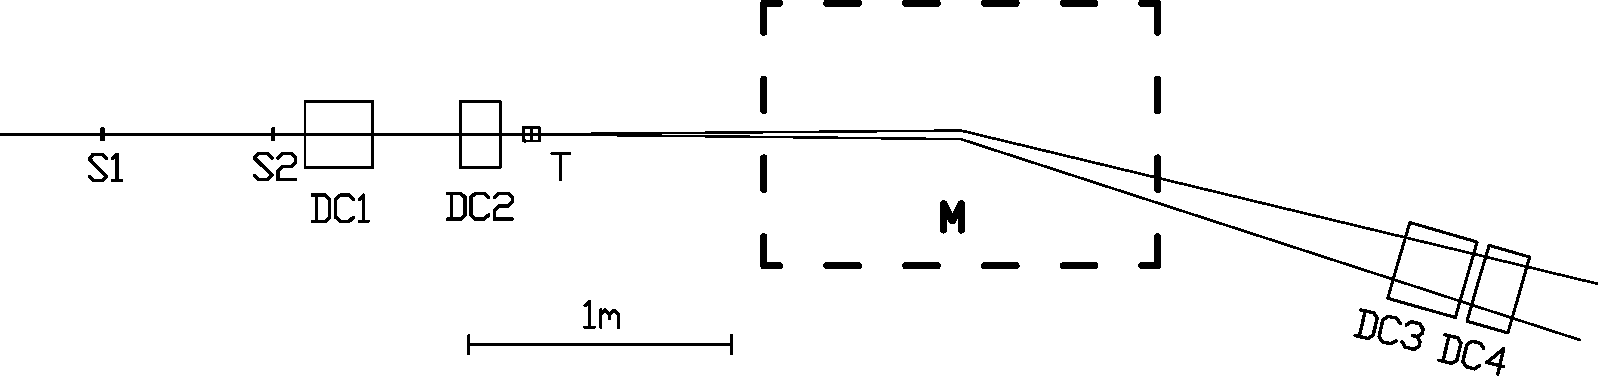
\includegraphics[width=1.00\textwidth]{STRELA_layout.pdf}
  \caption{Layout of the experimental setup for determining the spin-dependent
    part of \np scattering: scintillator counters S1 and S2, drift chambers (DC1
    -- DC4), analyzing magnet M and target T.}
  \label{fig:STRELA_layout}
\end{figure*}

The sensitive areas of the drift chambers are the following: 12.5 $\times$ 12.5
cm$^2$ for DC1, DC2 (small chambers) and 25 $\times$ 25 cm$^2$ for DC3, DC4 (large
chambers). The right handed coordinate system has been used, where the $z$ axis
is in the beam direction and $x$ and $y$ axis lie in the plane of the
chambers. All chambers contain an (Ar$_2$CH$_4$) gas mixture and have
alternating, orthogonal $x$ and $y$ coordinate planes. DC1 and DC3 are composed
of 8 sensitive planes ($4x$, $4y$) while DC2 and DC4 are composed of 4 sensitive
planes ($2x$, $2y$). The analyzing magnet M of field intensity $B = 0.85$ T is
used to separate deuterons and two protons, respectively.

The drift length for all chambers is $r_{max} = 21$ mm. The basic
characteristics of the drift chambers have been established from irradiation of
a polyethylene target with a deuteron beam of 3.5 \GeVc momentum. For each wire
the minimal $t_{min}$ and maximal $t_{max}$ drift times have been
determined. The average total drift time was found to be $\sim$~450~ns. In the
track finding procedure the relation between the measured drift time and the
minimal distance from the anode wire to the track plays an important role. To
find the function, transforming the drift time $t$ to radius $r$, also referred
to as $r(t)$ relation, is the central task. This transformation function may
depend on many parameters like: the electric field strength, the gas mixture,
the pressure, the temperature and the drift chamber geometry. For determination
of the transformation function two methods are applied: the linear or quick one,
mainly used for the preliminary results and online monitoring, the second
method, called cumulative or integral one suitable for offline purposes, which
gives the final results. The spatial resolution of the drift chambers used in
the STRELA setup is in the range of $\sim$~80\,--120~$\muup$m
% \muup (or \upmu) not for mathptmx
(Fig.~\ref{fig:res_chambers}). More technical details and the algorithm of the
track reconstruction can be found in \cite{gla13}.

\begin{figure}[ht]
  \centering
  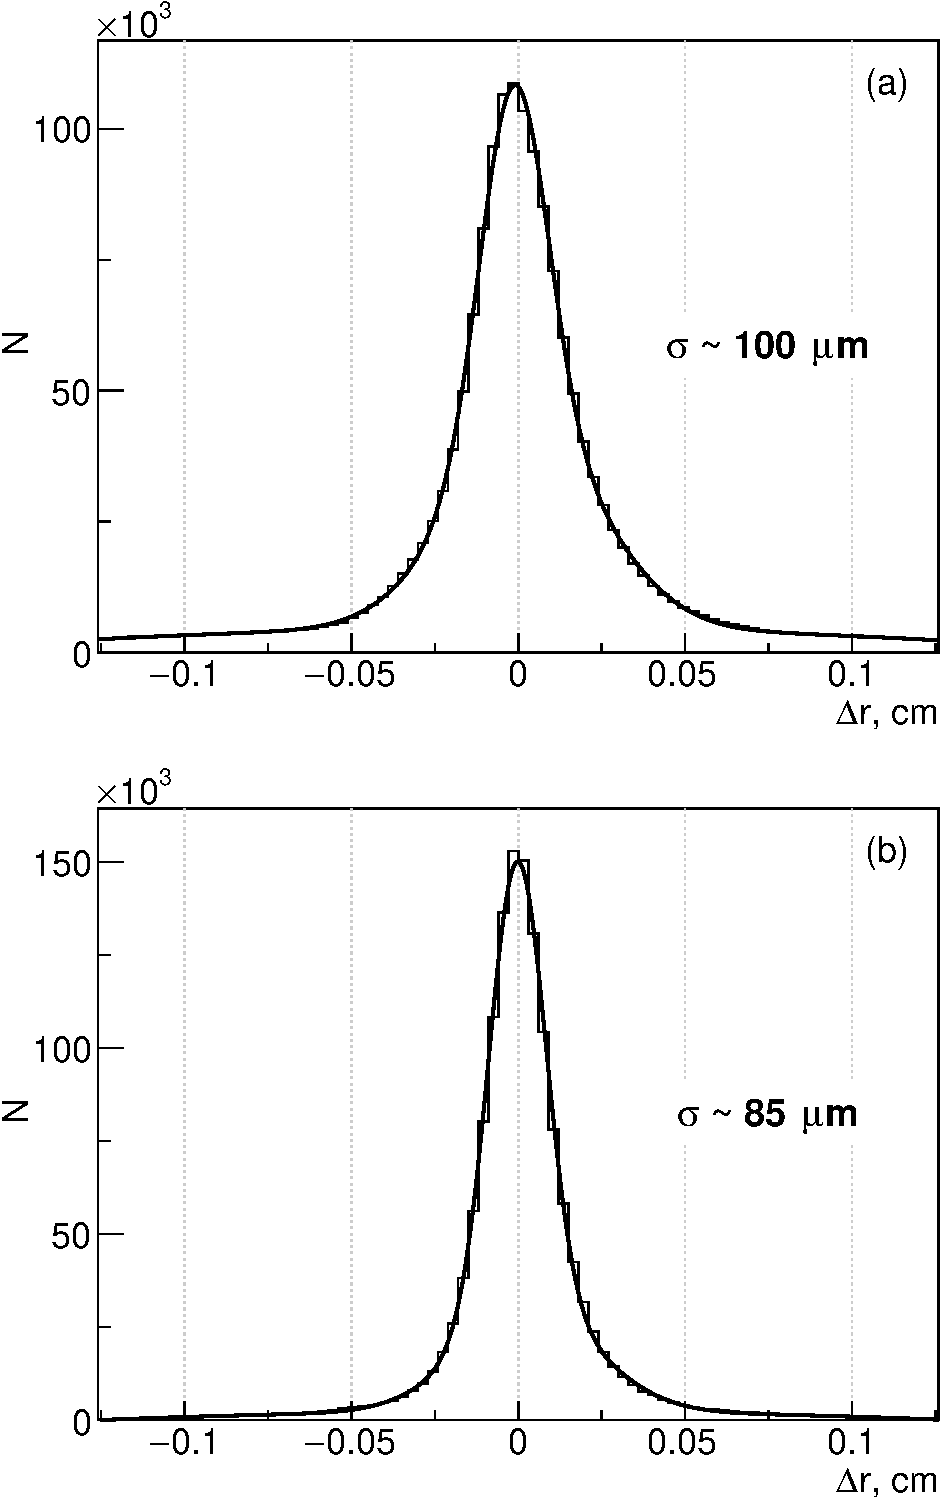
\includegraphics[width=0.48\textwidth]{res_chambers.pdf}
  \caption{Example of distribution of track residuals $\Delta r$ in the $xz$
    plane of drift chambers: (a) small and (b) large. The solid curve is a
    double Gaussian approximation.}
  \label{fig:res_chambers}
\end{figure}

The experimental setup was started by the two polysty\-rene based scintillation
counters S1 (dimensions 10 $\times$ 10 $\times$ 0.5 cm$^3$) and S2 (dimensions 7
$\times$ 7 $\times$ 0.5 cm$^3$). The light guides are made of plexiglass. For
light readout XP 2020 photomultipliers were used. The signals from the
photomultipliers are connected to the shaper inputs. The use of these shapers
allows to compensate the time spread of the signals caused by the leading edge
of the amplitude of the photomultiplier signal. The time and amplitude
information from the counters is digitized and recorded in each event for the
subsequent monitoring of the counters and the entire trigger system
functionality. The trigger system of the setup must ensure selection of events
of the deuteron breakup reaction at zero angle (or close to zero) between the
incoming deuteron and scattering protons. The acceptance of the experimental
facility for the studied process of charge exchange reaction is close to 100~\%.

The dipole electromagnet 2SP-40, with transverse dimensions 100 $\times$ 30
cm$^2$, was used as an analyzing magnet. The magnet creates the required
magnetic field in the range of \ 0.7\,--1.0 T at a distance of 150 cm along the
path of the particles. The spreads in space of the non interacting deuteron beam
and that of the recorded protons from the examined reaction are bended to the
blocks of large drift chambers for detection. The radius of the curvature of the
stripping protons trajectory in the magnet is about 7 m at the value of the
magnetic field 0.83 T.

The STRELA setup is irradiated with a deuteron beam of an incident momentum of
3.5 \GeVc. The detected events are supposed to contain either two protons with
close momenta (equal to the half of the incident deuteron beam momenta), from
the charge exchange reaction of a deuteron with a proton \dpchex or a single
proton from the charge retention deuteron breakup \dpret. The extracted beam
intensity from the accelerator is not lower then $\sim 10^{7}$ particles per
spill. Since the drift chambers are operable at intensities lower than
$\sim 10^{6}$ particles/spill, a steel collimator with a rectangular aperture of
4 $\times$ 4 mm$^2$ and a length of 1.2 m has to be used to reduce the
intensity. After applying the collimator the deuteron beam intensity of
$\sim 5\times10^5$ particles per spill or below is reached at the target. The
deuteron flux (number of triggers) has been determined using S1 and S2
scintillation counters (monitored numbers) in coincidence. This is corrected for
the efficiency of the drift chambers and admixture in the beam using a direct
deuteron beam. The track of deuteron beam in drift chambers DC1, DC2 before
magnet and behind DC3, DC4 are reconstructed using the track reconstruction
algorithm \cite{gla13}. The value of the correction is different from run to run
and is in the interval 0.85~--~0.89.

Carbon (C) and polyethylene (CH$_2$) targets have been used to extract the $dp$
interaction. The final distributions of the $dp$ interactions are obtained by
subtracting CH$_2$ and C distributions. The size of the targets have been
determined by carbon nuclei equivalent. Carbon target was used to account for
the background events. The shape of targets CH$_2$ and C are cylindrical, both
with diameters of 60 mm. The length of targets CH$_2$ and C are 48 mm and 54 mm,
respectively. The density of H nuclei per cm$^2$ for CH$_2$ target is (4.74
$\pm$ 0.05)$\times$10$^{23}$ ???/cm$^2$.
% co za jednotky, nie je to v poriadku ?!
The background from other channels of the $dp$ reaction and the influence of
carbon nuclei have been estimated by the use of the GEANT3 simulation package
for transporting the reaction products (taken from the corresponding events of
the one meter bubble chamber at the momenta 3.35 \GeVc) through the experimental
setup. More details about the chamber experiment can be found in
\cite{gla02,gla08}. There is also shown that the \dpchex reaction proceeding
predominantly as a quasi free nucleon interaction and intermediate isobaric
states does not influence the differential cross section at $t = 0$.

\section{Data analysis and experimental results}
The experimental facility has been irradiated in the beam of deuterons with 3.5
\GeVc momenta. In the last run of March 2014 one billion triggers were received.
The first step in the analysis was to decode events. Calibration procedure and
the track reconstruction in the drift chambers transformed the raw data into
physical quantities. For the further processing and physical analysis three
tracks in the $xz$ plane were selected: one before the target and two behind it.
The topology of this events is shown in Fig. \ref{fig:STRELA_layout}.

\begin{figure}[h]
  \centering
  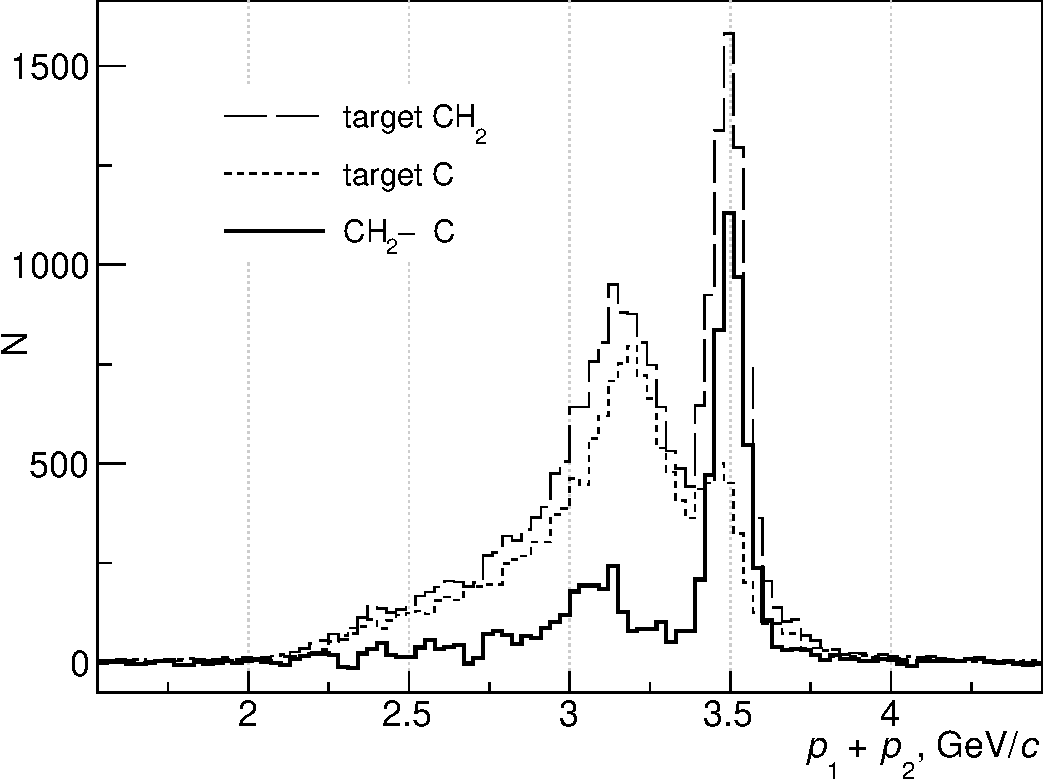
\includegraphics[width=0.48\textwidth]{p1_plus_p2_1.pdf}
  \caption{Distributions of the sum of the two protons momenta from $dp$
    reaction, experimental results: (a) target CH$_2$ red line, target C blue
    line, (b) difference between CH$_2-$\,C targets.}
  \label{fig:p1p2exp}
\end{figure}

The distribution of the sum of the two charged particles (two protons) momenta
for both targets are obtained. The background from C and CH$_2$ targets can be
neglected. The dependences of the sum of the two proton momenta from $dp$
reaction are presented in Fig. \ref{fig:p1p2exp} for CH$_2$ and C targets (a)
and their difference CH$_2-\,$C (b). The results of simulation
(Fig. \ref{fig:p1p2sim}) include all channels $dp$ reaction (a) and channel
\dpfrag only (b). Note that for simulation was used real events from the one
meter bubble chamber at the momenta 3.35 \GeVc (with relative small statistics).
As one can see, the distribution has a characteristic peak near the incoming
deuteron momentum kinematically associated with the pair of protons from the
\dpfrag reaction (Fig. \ref{fig:p1p2exp} (b)). The contribution from the
background reactions, other than the studied \dpfrag reaction, which could also
produce the two positively charged track in the forward direction, is negligible
(Fig. \ref{fig:p1p2sim} (b)). Into the differential cross section $d\sigma/dt$
% for \dpchex reaction
only those events have been included, where the sum of the two charged particle
momenta is in the interval (3.5 $\pm$ 0.2) \GeVc (Fig. \ref{fig:p1p2exp} (b)).

\begin{figure}[h]
  \centering
  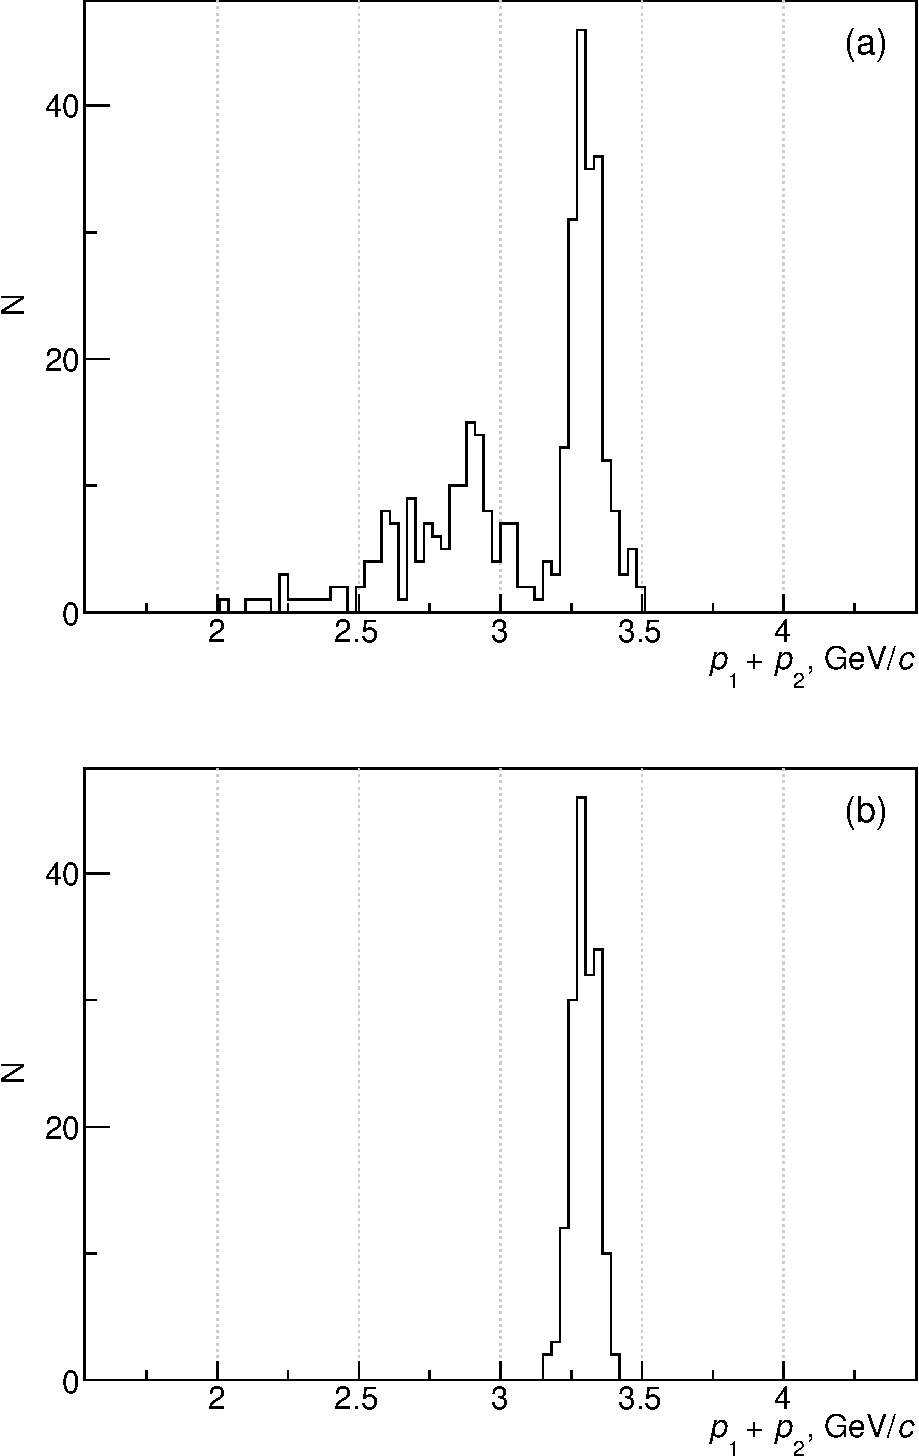
\includegraphics[width=0.48\textwidth]{p1_plus_p2_2.pdf}
  \caption{Distributions of the sum of the two protons momenta from $dp$
    reaction, simulation results: (a) include all channels $dp$ reaction and (b)
    channel \dpfrag only.}
  \label{fig:p1p2sim}
\end{figure}

The plot of momenta $p_1$ \textit{vs.} $p_2$ of the two charged particles (two
protons) from $dp$ reaction is shown in Fig. \ref{fig:p1vsp2}. From comparison
simulation results (a) and (c) with experimental results (b), it can be seen
that the background from other channels of the $dp$ reaction may be eliminated,
extracted.

\begin{figure}[t]
  \centering
  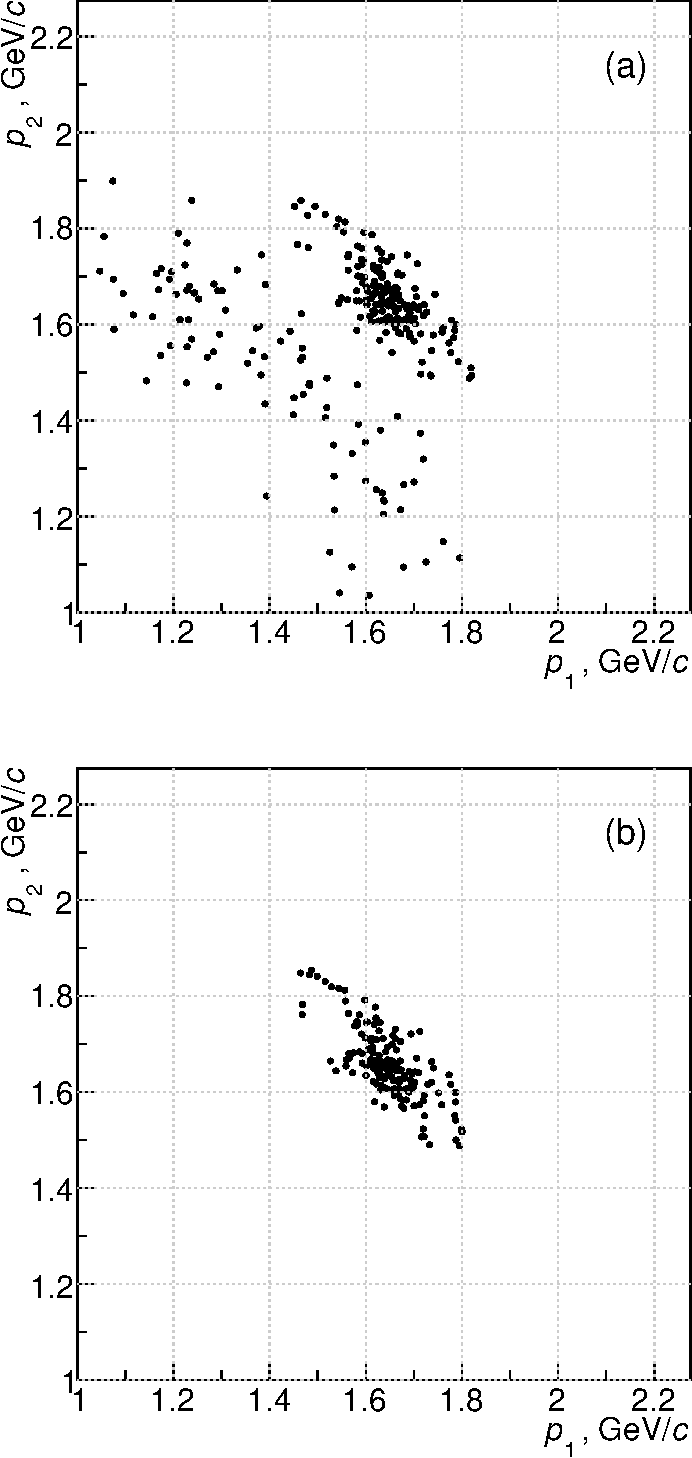
\includegraphics[width=0.41\textwidth]{p1_vs_p2_1.pdf} % maximum width=0.41
  \caption{Two dimensional distribution of the measured momenta $p_1$
    \textit{vs.} $p_2$ of the two protons from $dp$ reaction: (a) simulation
    includes all channels $dp$ reaction, (c) simulation only \dpfrag channel and
    (b) experimental distribution.}
  \label{fig:p1vsp2}
\end{figure}

The measured differential distribution $dN\,/\,dt$ of the \dpchex reaction is
displayed in Fig. \ref{fig:dndt} together with the curve corresponding to fit by
expression
\begin{equation}
  \label{eq:dndtfit}
  dN/dt = a\,\exp(b\,t)\,,
\end{equation}
with parameters $a=(435.6\,\pm\,6.8)$ and $b=(-440.9\,\pm\,9.1)$. Extrapolation
to $t=0$ gives $(dN/dt)|\,_{t=0}=(435.6\,\pm\,6.8)$ N$/$(\GeVc)$^{\,2}$. This
value corresponds to a value of the charge exchange reaction differential cross
section $(d\sigma/dt)|\,_{t=0}=(30.56\,\pm\,0.48$) mb$/$(\GeVc)$^{\,2}$. The
quoted error is statistical only. Systematic uncertainties which affect the
overall normalization of the cross sections have been estimated to be about
5~\%. This uncertainty stems mainly from the deuteron flux determination. The
uncertainty from the target thickness and the histogram bin width are comparably
small.

\begin{figure}[h]
  \centering
  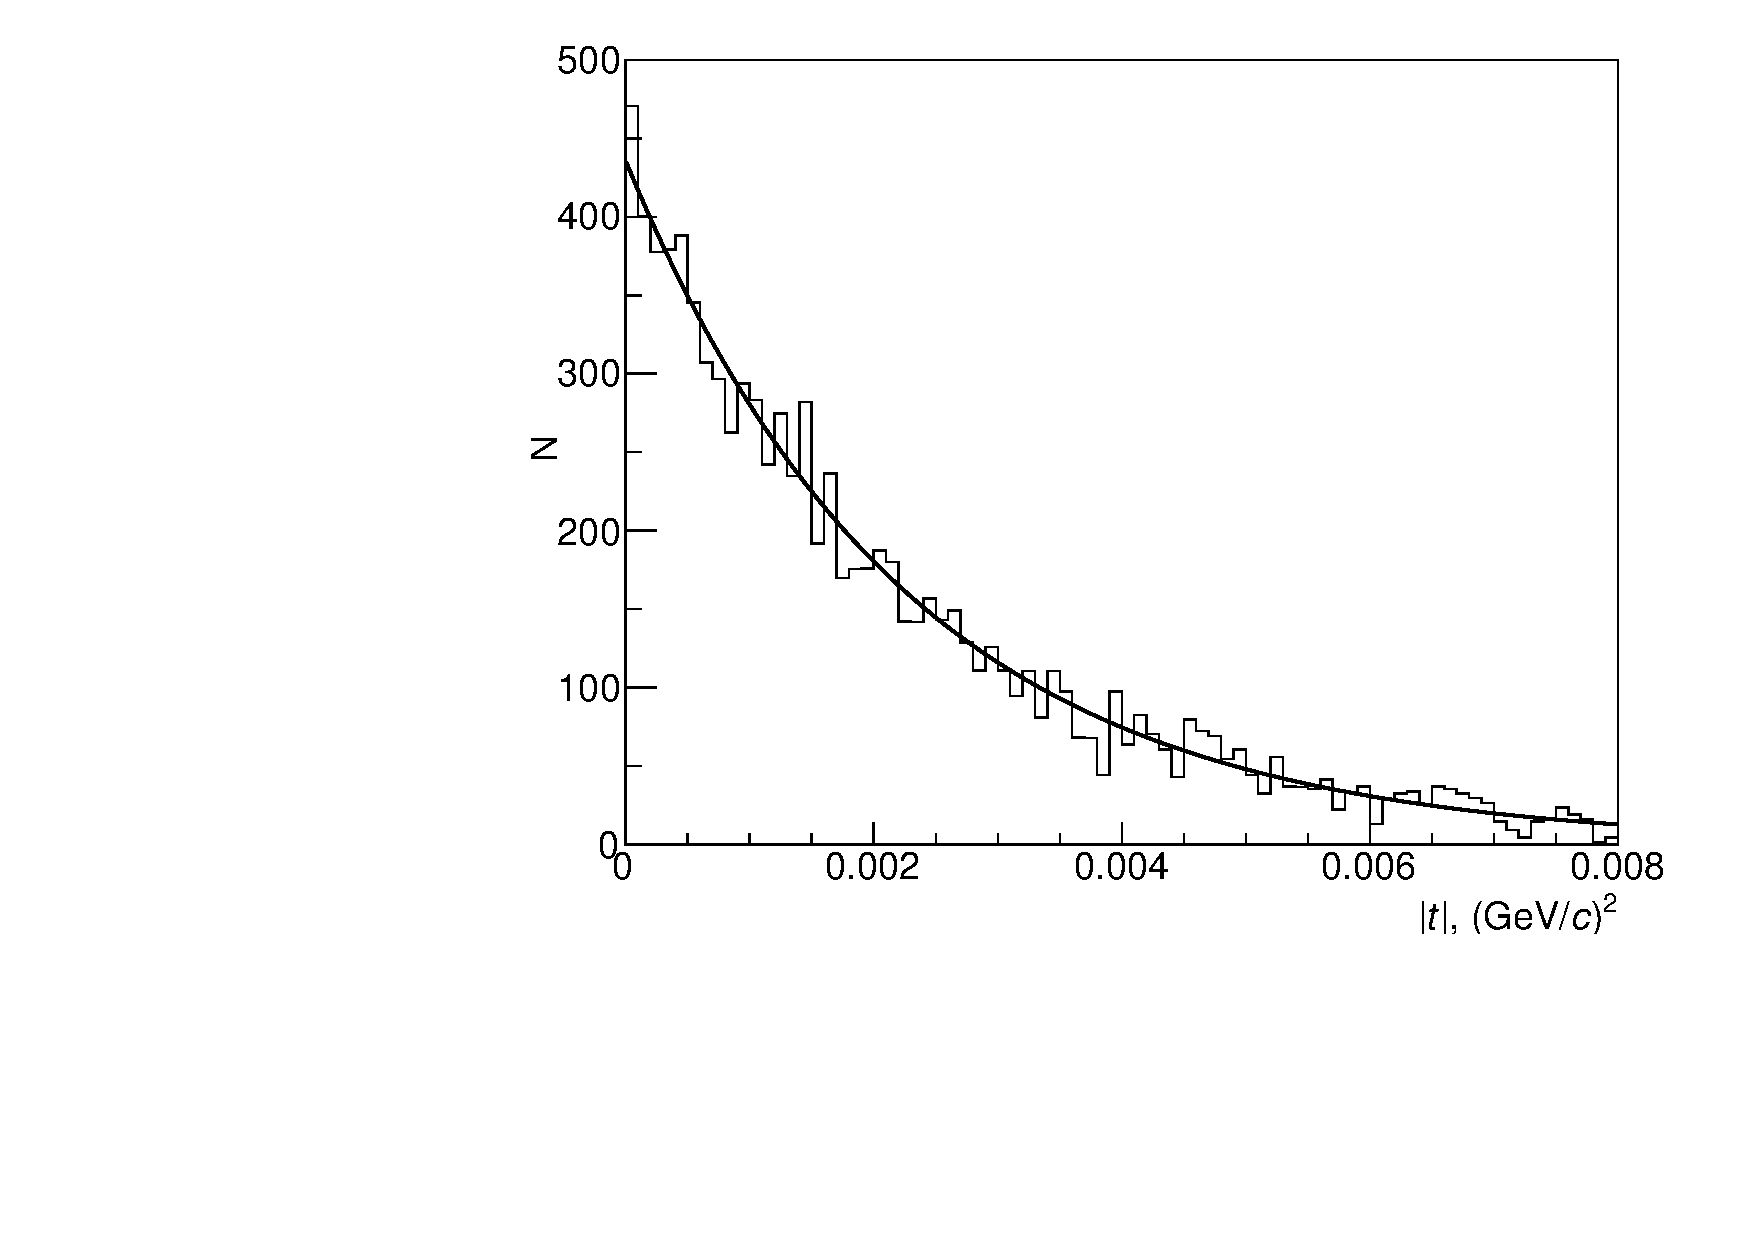
\includegraphics[width=0.48\textwidth]{dp_dN.pdf}
  \caption{Differential distribution $dN/dt$ of the \dpchex reaction. The solid
    line is approximation by Eq. \eqref{eq:dndtfit}, see details in the text.}
  \label{fig:dndt}
\end{figure}

The cross section was calculated using the relation
\begin{equation}
  \sigma =
  \frac{1}{n\,lb_w}\ln\bigg(1\Big/\Big(1-\frac{N_{int}}{N_0}\Big)\bigg)\,,
  %  \sigma =
  %  \frac{1}{n\,lb_w}\ln\left(1\middle/\left(1-\frac{N_{int}}{N_0}\right)\right)
\end{equation}
where $n$ is the concentration of H nuclei ?!in cm$^3$?! in target, $l$ is the
target length, $b_w$ is the histogram bin width, $N_{int}$ is the number of
interactions and $N_0$ is the number of beam triggers. The number of triggers is
corrected for the efficiency of chambers.

The obtained charge exchange differential cross section on the deuteron at $t=0$
was compared with the available data from \np reaction at the same interpolated
energy from published data. The closest energy data comes from measurements made
at the SATURN accelerator \cite{biz75,bys78}. Unlike to the other similar
experiments, Bizard et al. \cite{biz75} used quasi monochromatic neutrons from
accelerated deuteron stripping with a momentum spread of 5~\%. New data about
\np scattering at the momenta of incident quasi monochromatic neutrons at 1.43,
2.23 and 5.20 \GeVc have been obtained in \cite{tro14}.

The values of $(d\sigma/dt)|\,_{t=0}$ of \np reaction as a function of the
incident momenta is shown in Fig. \ref{fig:npsigma}. Each individual
differential cross sections from Bizard et al. \cite{biz75} are transformed into
$d\sigma/dt$ versus $t$ in the region of momenta 1.4~--~2.0 \GeVc and
extrapolated at each momentum to $t=0$ by fitting the expression
$d\sigma/dt = a\,\exp(b\,t + c\,t^2)$. %in interval $t < 0.01$ \GeVc.

\begin{figure}[ht]
  \centering
  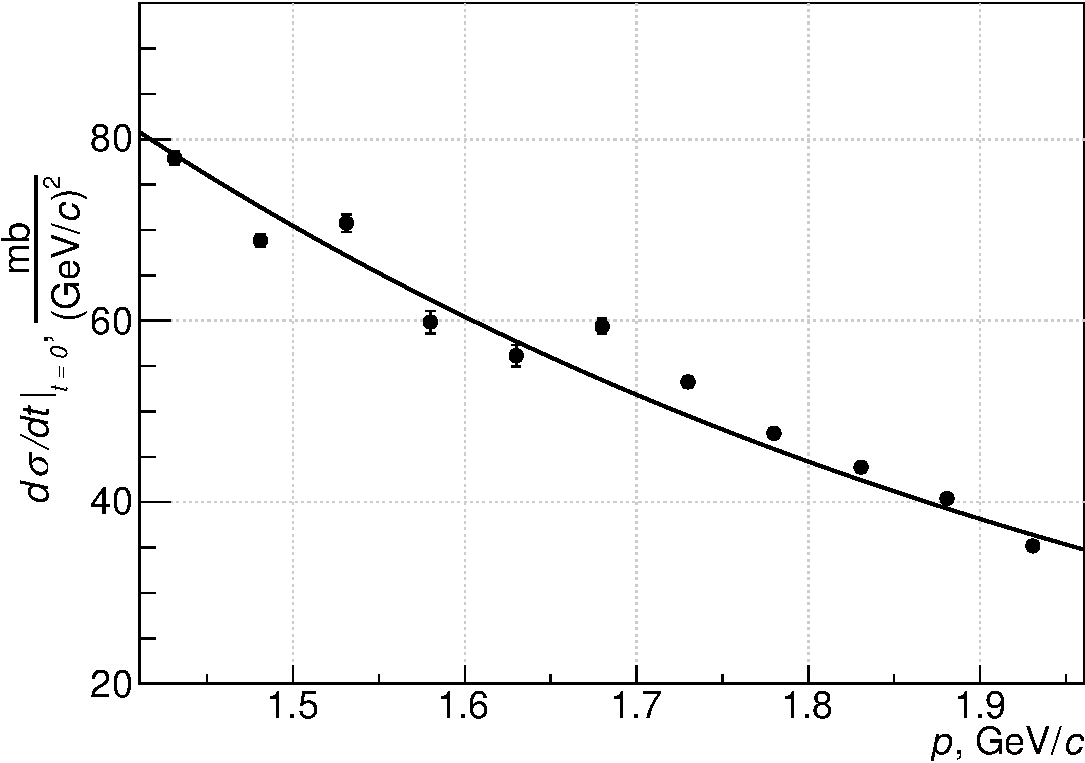
\includegraphics[width=0.48\textwidth]{np_dSigma.pdf}
  \caption{The dependence of the $(d\sigma/dt)|\,_{t=0}$ for the \np reaction on
    the beam momentum. The data points are computed from the experimental
    results \cite{biz75}. The solid curve is a simple exponential fit to the
    data points.}
  \label{fig:npsigma}
\end{figure}

To determine the $(d\sigma/dt)|\,_{t=0}$ of the \np reaction at ``our incident''
proton momentum of 1.75 \GeVc/nucleon, an exponential fit is made to the results
of Fig. \ref{fig:npsigma}, which gives the following value of
$(d\sigma/dt)|\,_{t=0} = (48.0\,\pm\,0.2$) mb$/$(\GeVc)$^{\,2}$. The systematical
error due to fit procedure is approximately 5~\%. The obtained value will be
related to the estimated differential cross section of the quasi elastic \dpchex
charge exchange at $t=0$ from our experiment.

One can introduce the ratio of the differential cross sections for the forward
scattering (charge exchange) on the deuteron and proton
\begin{equation}
  \begin{split}
    R_{\np} &= \frac{(d\sigma/dt)_{\dpchex}}{(d\sigma/dt)_{\np}} \\
    &= 0.64 \pm 0.01\,\mathrm{(stat.)} \pm 0.04\,\mathrm{(syst.)}.
  \end{split}
\end{equation}
Under the assumption Eq. \eqref{eq:dp_23np} and Eq. \eqref{eq:np_sum} stated
above this, $R_{\np}$ can be related to
\begin{equation}
  R_{\np} = \frac{2}{3}\,\frac{(d\sigma/dt)^{SD}_{\np}}{(d\sigma/dt)_{\np}}
\end{equation}
and accordingly the value of the spin-independent part of the elastic \np charge
exchange cross section has been obtained as
\begin{equation}
  \begin{split}
    R^{\,ID}_{\np} &= \frac{(d\sigma/dt)^{SI}_{\np}}{(d\sigma/dt)^{SD}_{\np}}
    = \frac{2}{3\,R_{\np}} \ - \ 1 \\
    &= 0.05 \pm 0.02\,\mathrm{(stat.)} \pm 0.07\,\mathrm{(syst.)}.
  \end{split}
\end{equation}
It should be emphasized that the obtained contribution, of course, depends on
the elementary \np charge exchange cross section which is taken from another
experiment and on the systematical errors of approximately 5~\% which is due to
the fit procedure. Preliminary data have been published in \cite{bas14,bas16}.

\section{Conclusion}
The spectrometric complex has been developed on the basis of the STRELA setup to
study the charge exchange reaction in unpolarized deuteron beam. The value of
the charge exchange reaction \dpchex differential cross section
$(d\sigma/dt)|\,_{t=0}=(30.56\,\pm\,0.48$) mb$/$(\GeVc)$^{\,2}$ has been
obtained at 1.75 A \GeVc. The obtained ratio of the charge exchange differential
cross sections at \dpchex at $t=0$ for \dpchex and \np reactions
$R_{\np} = 0.64 \pm 0.01\,\mathrm{(stat.)} \pm 0.04\,\mathrm{(syst.)}$ testifies
the prevailing contribution of the spin-dependent part to the \np cross section
scattering. The obtained ratio depends on the $(d\sigma/dt)|\,_{t=0}$ the \np
reaction extracted from published data. Continuation of these researches at
higher energies on STRELA setup is in progress.

\begin{acknowledgements}
  The authors are grateful to the JINR VBLHEP directorate for supporting their
  experiment and the Nuclotron accelerator team. This research was supported by
  the Ministry of Education, Science, Research and Sport of the Slovak Republic
  (VEGA Grant No.~1/0113/18).
\end{acknowledgements}

\begin{thebibliography}{99}
\bibitem{pom51}
  I. Pomeranchuk, Sov. JETF \textbf{21}, 1113 (1951)
\bibitem{chew51}
  G.F. Chew, Phys. Rev. \textbf{84}, 710 (1951)
\bibitem{mig55}
  A.B. Migdal, J. Exp. Theor. Phys. (in Russian) \textbf{28}, 3 (1955)
\bibitem{pom51_2}
  I. Pomeranchuk, Dokl. Akad. Nauk (in Russian) LXXVIII, 249 (1951)
\bibitem{lap57}
  L.I. Lapidus, J. Exp. Theor. Phys. (in Russian) \textbf{32}, 1437 (1957)
\bibitem{dea72}
  N.W. Dean, Phys. Rev. D \textbf{5}, 1661 (1972)
\bibitem{dea72_2}
  N.W. Dean, Phys. Rev. D \textbf{5}, 2832 (1972)
\bibitem{ala75}
  B.S. Aladashvili et al., Nucl. Phys. B \textbf{92}, 189 (1975)
\bibitem{ala75_2}
  B.S. Aladashvili et al., Nucl. Phys. B \textbf{86}, 461 (1975)
\bibitem{bug87}
  D.V. Bugg, C. Wilkin, Nucl. Phys. A \textbf{167}, 575 (1987)
\bibitem{led04}
  R. Lednicky, V.L. Lyuboshitz, V.V. Lyuboshitz, Proc. ISHEPP XVI, 199,
  Dubna (2004)
\bibitem{gla02}
  V.V. Glagolev et al., Eur. Phys. J. A \textbf{15}, 471 (2002)
\bibitem{gol66}
  M. Goldberger, K. Watson, Collision Theory, Wiley, New York (1966)
\bibitem{gla08}
  V.V. Glagolev et al., Cent. Eur. J. Phys. \textbf{6}, 781 (2008)
\bibitem{gla13}
  V.V. Glagolev et al., Instrum. Exp. Tech. \textbf{56}, 387 (2013)
\bibitem{sha09}
  V.I. Sharov et al. Eur. Phys. J. A \textbf{39}, 267 (2009)
  % https://doi.org/10.1140/epja/i2008-10719-x
\bibitem{sha09_2}
  V.I. Sharov et al., Phys. At. Nucl. \textbf{72}, 1007 (2009) \\ % !!!
  V.I. Sharov et al., Phys. At. Nucl. \textbf{72}, 1021 (2009)
  % https://doi.org/10.1134/S1063778809060131
  % https://doi.org/10.1134/S1063778809060143
\bibitem{shi11}
  R.A. Shindin et al., Phys. Part. Nucl. Lett. \textbf{8}, 90 (2011)
  % https://doi.org/10.1134/S1547477111020129
\bibitem{biz75}
  G. Bizard et al., Nucl. Phys B \textbf{85}, 14 (1975)
\bibitem{bys78}
  J. Bystricky, F. Lehar, Nucleon-Nucleon Scattering data, Karlsruhe:
  Fachinformationszentrum, 521, (1978)
\bibitem{tro14}
  Yu.A. Troyan et al., Phys. Part. Nucl. Lett. \textbf{11}, 101 (2014)
\bibitem{bas14}
  S.N. Basilev et al., PoS (Baldin ISHEPP XXII), 137, 2014
\bibitem{bas16}
  S.N. Basilev et al., J. Phys. Conf. Ser. \textbf{678}, 012040, 2016
\end{thebibliography}

\end{document}

%%% Local Variables:
%%% mode: latex
%%% TeX-master: t
%%% End:
